\section{Simulation Results}
\label{sec:simulations}

In this section, we present two simulation scenarios in which the \textit{LinDist3Flow} equations have been incorporated into OPF formulations. The first experiment considers the dispatch of DER resources to minimize feeder-head real power.  The results of the OPF are compared to an alternative optimization approach using convex relaxations and semidefinite programming.  The second experiment considers the dispatch of DER resources to regulate and balance feeder voltages.  

Both experiments were conducted on the IEEE 13 node distribution feeder model \cite{IEEEtestfeeder}, the topology of which is shown in Fig. \ref{fig:13node}.  While we have tested both scenarios on larger feeders models, in this work we have chosen to present results for the IEEE 13 node feeder for clarity of presentation and for the large amount of voltage imbalance between phases. In the simulations, feeder topology, line configuration, line impedance, line length, and spot loads are specified in \cite{IEEEtestfeeder}. Delta to Wye conversions were performed where appropriate. Furthermore, our simulations omitted the voltage regulator between nodes 650 and 632, the transformer between nodes 633 and 634, the switch (assumed closed) between nodes 671 and 692, and capacitors at nodes 675 and 611. Spot loads were increased by a factor of 1.25 to increase voltage imbalance. Finally, four-quadrant-capable DER were placed at the following nodes: 632, 675, 680, and 684. We assume each DER has 3 phase control and can inject or sink both real and reactive power separately on each phase of the feeder.  The DER are constrained by an apparent power capacity limit on each phase of 250 kVA, or 0.05 pu.  In both experiments, voltage magnitudes were constrained to be within $\pm 5\%$ of 1.0 p.u. The voltage at the feeder head was assigned as: $\mathbb{V}_{0}$ = [$1\angle 0\degree$,  $1\angle 240 \degree$, $1\angle 120 \degree$]$^{T}$ p.u. for phases $a$, $b$, and $c$, respectively.

% \setlength{\belowcaptionskip}{-15pt}
% \setlength{\textfloatsep}{-15pt}
\begin{figure}[t]
	\centering
	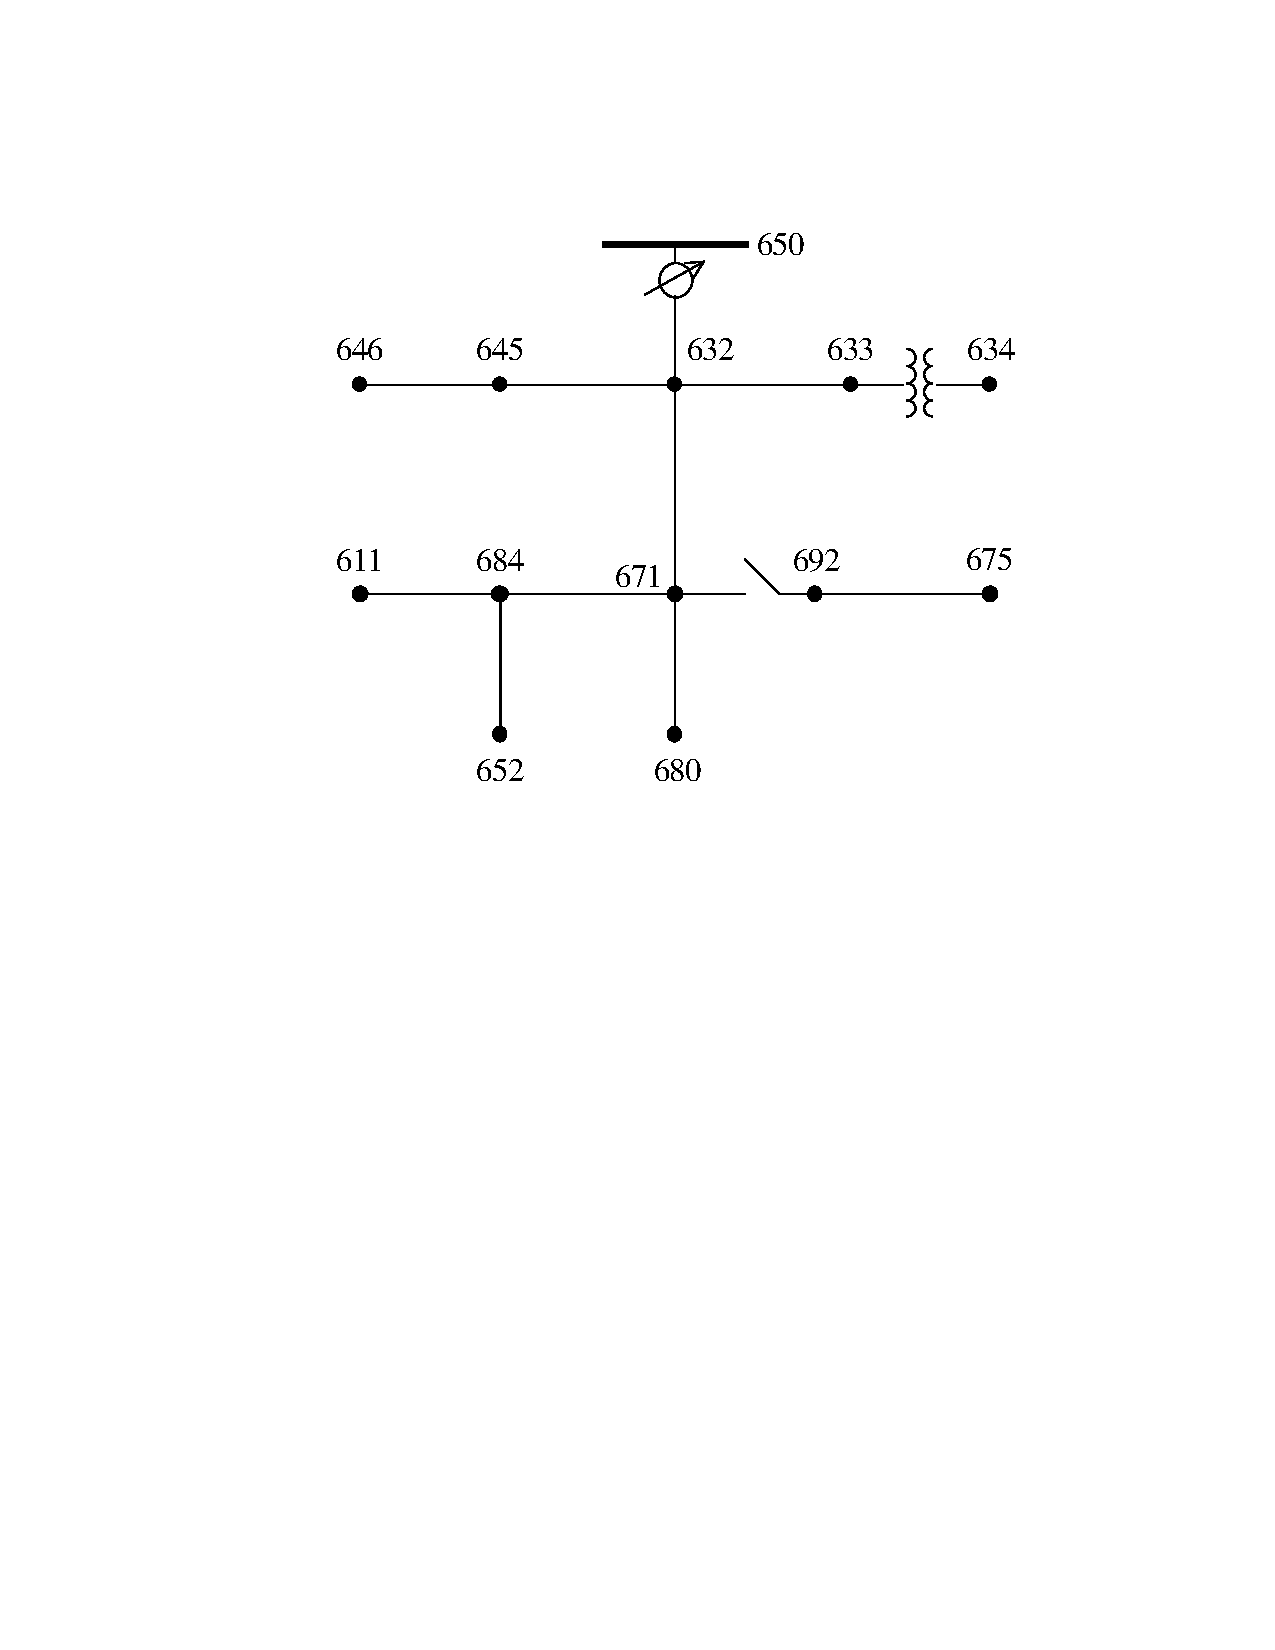
\includegraphics[width=0.45\textwidth]{13_node_feeder.pdf}
	\caption{IEEE 13 node feeder model.}
	\label{fig:13node}
\end{figure}

Figure \ref{fig:s2bc} shows the feeder voltage magnitude profile without any applied control (i.e. this is the ``no control" scenario in both experiments). In this and all subsequent figures, phase $a$ is depicted in red, phase $b$ is depicted in green, and phase $c$ is depicted in blue. Fig. \ref{fig:s2bc} highlights the large amount of voltage magnitude imbalance as well as violations of minimum voltage magnitude constraints on phase c.

% \begin{figure}[t]
% 	\centering
% 	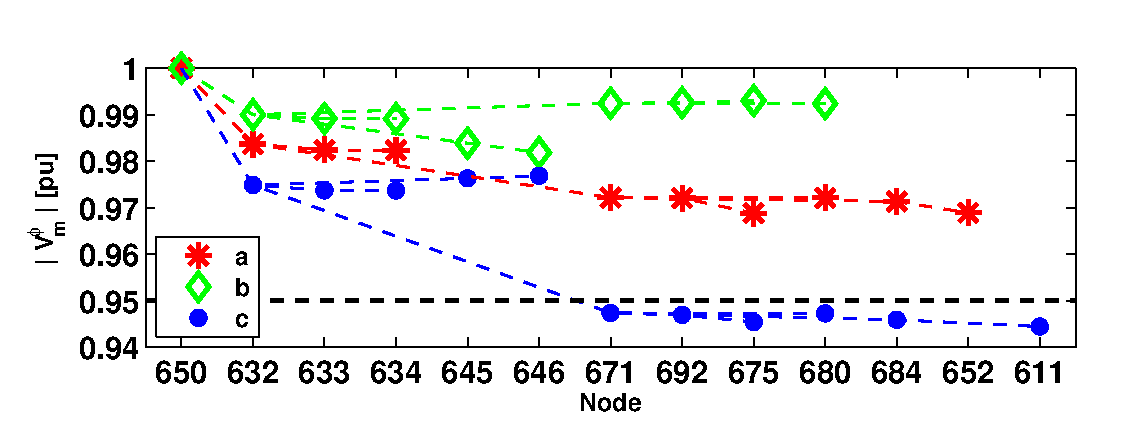
\includegraphics[width=0.49\textwidth]{s2bc.eps}
% 	\caption{Voltage profile of IEEE 13 node feeder without any DER control.}
% 	\label{fig:s2bc}
% \end{figure}

